\documentclass[11pt, oneside]{article} 
\usepackage{geometry}
\geometry{letterpaper} 
\usepackage{graphicx}
	
\usepackage{amssymb}
\usepackage{amsmath}
\usepackage{parskip}
\usepackage{color}
\usepackage{hyperref}

\graphicspath{{/Users/telliott_admin/Tex/png/}}
% \begin{center} 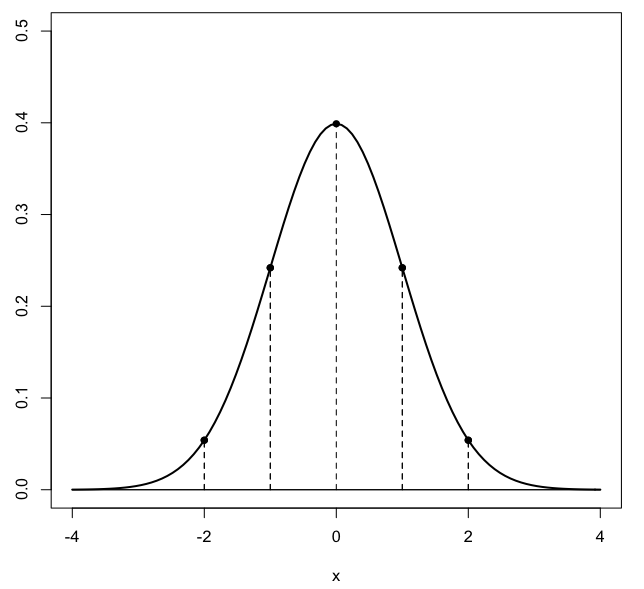
\includegraphics [scale=0.4] {gauss3.png} \end{center}

\title{Induction}
\date{}

\begin{document}
\maketitle
\Large

\label{sec:Induction}

In the figure below we have a polygon---an irregular heptagon.  Actually, there are three polygons altogether, there is the heptagon with $n+1$ sides, the hexagon with only $n$ sides that would result from cutting along the dotted line, and the triangle that is cut off.

What we would like to do is to find a formula for the sum of the internal angles that depends only on the number of sides or vertices.

\begin{center} 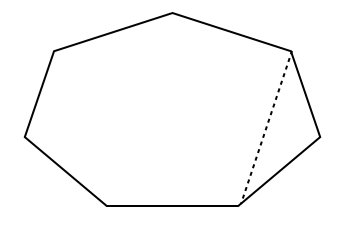
\includegraphics [scale=0.5] {polygon.png} \end{center}

The first part of the answer is to guess.  In the figure, you can see that by adding the extra vertex to go to the $n+1$-gon, we added a triangle, or perhaps you'd rather say than in going from $n+1$ to $n$ we lost a triangle.  

In either case, the difference is $180^\circ$.  The difference between having $n$ sides and $n+1$ sides is to add $180^\circ$.  

The second part of the argument is to suppose that $n=3$, in that case we must have simply $180^\circ$ degrees for a triangle.  So we guess that the formula may be
\[ (n-2)180^\circ = S_n \]
where S is the sum of the angles in an $n$-gon.

We can use induction to prove that this formula is correct.

The proof has two parts.  We must verify the formula for a base case like the triangle, which we've done.  You may wish to check that it works for the square as well, but that's not strictly necessary.

The second part of the proof is to verify that in going from $n$ to $n+1$, we add another $180^\circ$.  \[ (n-2)180^\circ + 180^\circ \stackrel{?}{=} ((n+1)-2)180^\circ \]
On the left-hand side, we have the sum of angles for $n$ sides, which we assume is correct, and then we just add $180^\circ$ to it.  On the right, we have substituted $n+1$ into the formula.

Now we need to show that these are equivalent.  But of course
\[ (n-2)x + x = ((n+1)-2) x \]
\[ n - 2 + 1 = n + 1 - 2 \]
$\square$

That is the inductive proof of the formula.

We can visualize an inductive proof as a kind of chain.  We showed that the "base case" is true, for n = 3.  We also showed that if the formula works for n (when plugging into $n-2(180)=S$), it must work for n+1.

\begin{quote}Mathematical induction proves that we can climb as high as we like on a ladder, by proving that we can climb onto the bottom rung (the basis) and that from each rung we can climb up to the next one (the step).\end{quote}

- Graham, Knuth and Patashnik

\subsection*{sums of integers}

To compute Riemann sums, we need to find formulas for several sums.  

To keep it simple, let's start with finite sums like the integers from $1$ to $n$
\[  1 + 2 + 3 + \cdots + n  \]
The numbers we seek are called the triangular numbers.  These are
\[ 1, 3, 6, 10, 15 \cdots \]
Here is a striking "visual proof" of the formula to obtain T$_n$, the $n^{th}$ such number.  The total number of circles in the figure below is $n \times (n+1)$ and this is exactly two times the sum of the integers from $1$ to $n$.

\begin{center} 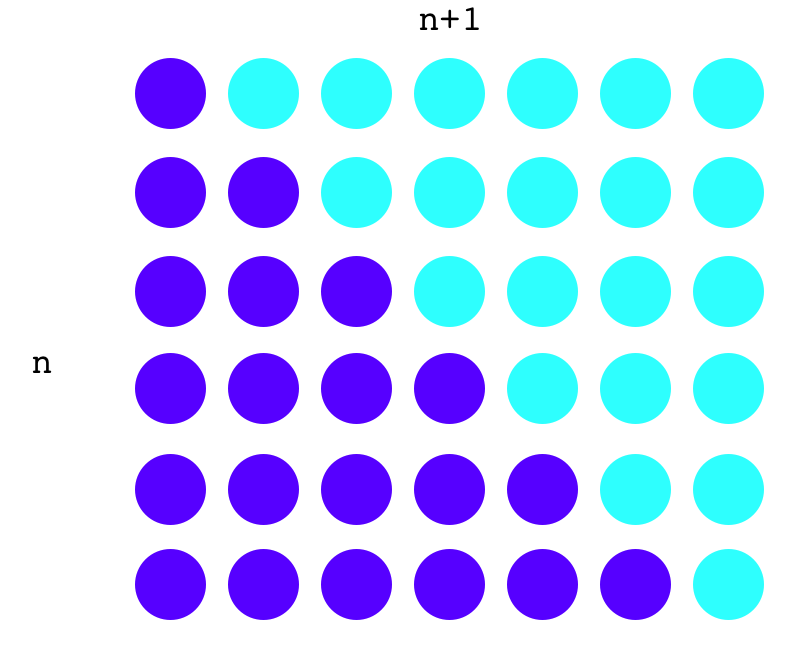
\includegraphics [scale=0.25] {sum_n.png}\end{center}
\[ 2S = n(n+1) \]
There is a famous story about Gauss that, as a schoolboy, he "saw" how to add the integers from $1$ to $100$ as two parallel sums
\[ \ \  1 + \ \ 2 + \ \ 3 + \cdots + 99 + 100 \]
\[ 100 + 99 + 98 + \cdots + 2 + 1 \]
Added together horizontally, these two series must equal twice the sum of $1$ to $100$.  But in the vertical, we notice that we have $n$ sums, each of which is equal to $n+1$.  So, again
\[ 2S = n (n+1) \]
\[ S = \frac{1}{2} \ n (n+1) \]
For $n=100$ the value of the sum is $5050$.  Another way of looking at this result is that between $1$ and $100$ there are $100$ representatives of the "average" value in the sequence, which (because of the monotonic steps) is $(100 + 1)/2 = 50.5$.  

Or alternatively, view the sum as ranging from $0$ to $100$ (with the same answer).  Now there are $101$ examples of the average value ($100 + 0)/2 = 50$).

\subsection*{Proof of the formula $n(n+1)/2$ by induction}

Returning to the sum of integers, one proof follows the method of induction.  In this approach, however, one must first guess the correct formula.  We guess $n(n+1)/2$, of course.  

Now, we \emph{assume} that the answer is correct for $n$.
\[ S_n = \frac{n(n+1)}{2} \]
So clearly, if $S_n$ is correct, then
\[ S_{n+1} = S_n + (n + 1) \]
Follow out the arithmetic:
\[ = \frac{n(n+1)}{2} + \frac{2(n+1)}{2} \]
\[ = \frac{n(n+1) + 2(n+1)}{2} \]
\[ = \frac{(n+1)(n+2)}{2} \]

But this is precisely what we would obtain by using the formula, and substituting $n+1$ for $n$.  Hence the formula gives the correct result for $n+1$, assuming that it gives the correct result for $n$.  In turn, it gives the correct result for $n$, assuming it gives the correct result for $n-1$.  Eventually, we reach the base case, where we can actually verify that the result is correct.

Try it on the first value in the sequence (the "base case").
\[ \frac{1(1+1)}{2} = 1 \]
That checks.  So the whole chain of reasoning is correct.  $\checkmark$

\subsection*{Derivation using sums}
It seems a shame to spoil such a beautiful proof "without words" as the one above by saying anything more, but I can't resist.  

You will notice that we were given the formula and only proved it true.  As we quoted Archimedes in the first chapter

\begin{quote}it is of course easier, when we have previously acquired by the method some knowledge of questions, to supply the proof than it is to find the proof without any previous knowledge.\end{quote}

I'd like to derive the equation we have been using using algebra.  The general method can be used to get the sum of the squares of integers, or their cubes, or even higher powers.

For any number $k$ it is true that
\[ (k+1)^2 = k^2 + 2k + 1 \]
So consider what happens if we sum the values from $k=1 \rightarrow n$ for each of these terms
\[ \sum_{k=1}^n (k+1)^2 = \sum_{k=1}^n k^2 + \sum_{k=1}^n 2k + \sum_{k=1}^n 1 \]

If the equation is valid for any individual $k$, then it is also true adding the equations for all $k$ from $1$ up to $n$.

Rearranging
\[ \sum_{k=1}^n (k+1)^2 - \sum_{k=1}^n k^2 = \sum_{k=1}^n 2k + \sum_{k=1}^n 1 \]
Now think about the left-hand side in our equation. 
\[ \sum_{k=1}^n (k+1)^2 - \sum_{k=1}^n k^2 \]
If we count down rather than up, start with $k=n$.  We have the following terms
\[ k = n \ \ \text{gives} \ \ (n+1)^2 - (n)^2 \]
\[ k = n-1 \ \ \text{gives} \ \ (n)^2 - (n-1)^2 \]
\[ k = n-2 \ \ \text{gives} \ \  (n-1)^2 - (n-2)^2 \]
\[ \cdots \]
\[ k = 1 \rightarrow \ \ (2)^2 - (1)^2 \]

We must add all of these together.  But notice how all the terms except the first and last cancel.  For example we have $-(n)^2$ in the top line and $(n)^2$ in the second. This is called a "collapsing" or "telescoping" sum.  We obtain
\[ S = (n+1)^2 - 1 \]\

Bringing back the right-hand side  we have
\[ (n+1)^2 - 1 = \sum_{k=1}^n 2k + \sum_{k=1}^n 1 \]

We can bring the constant factor $2$ out of the sum, and also, we recognize that the sum of the value $1$ a total of $n$ times is just $n$.
\[ (n+1)^2 - 1 = 2\sum_{k=1}^n k + n \]

Subtract $n$ from both sides.  The left hand side is
\[ (n+1)^2 - 1 - n = n^2 + n = n(n+1) \]
Finally, divide by $2$:
\[ \sum_{k=1}^n k = \frac{n (n+1)}{2} \]
That's our formula.

There is much more (sum of squares, cubes and so on) in the next chapter.
\subsection*{Odd number theorem}

Here is a simple but very useful inductive proof.

The \emph{odd number theorem} says that the sum of the first $n$ odd numbers is equal to $n^2$.  Here is a "proof without words".

\begin{center} 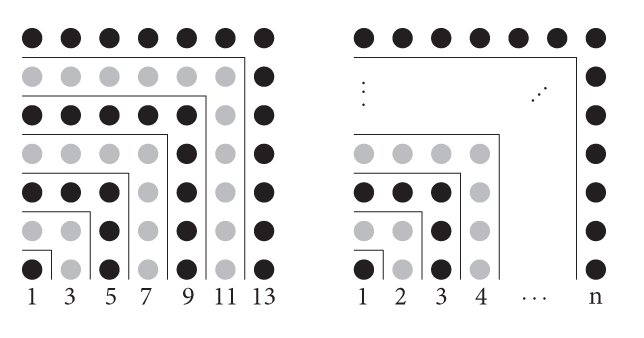
\includegraphics [scale=0.4] {odd_number_theorem.png} \end{center}

We prove this by induction.

\[ \ (0 \times 2 + 1) +  (1 \times 2 + 1) + (2 \times 2 + 1) + (\dots \]
\[ \dots + (n-1) \times 2 + 1) = n^2 \]

Notice that the $n$th odd number is $2 \times (n-1) + 1$.

Our formula says that
\[ 1 + 3 + 5 + \dots + (2n - 1) = n^2 \]
If you like the summation style:
\[ \sum_{k=0}^n 2k - 1 = k^2 \]

As an example, the first five odd numbers are
\[ 1 + 3 + 5 + 7 + 9 = 25 = 5^2 \]

So, if we consider the next odd number, $n$ changes to $n+1$.  The left-hand side gets another term:  we add $2 \times (n+1)-1$ to it.  That is equal to $2n + 1$.

To maintain the equality, add the same quantity to the right-hand side:
\[ n^2 + 2n + 1 = (n+1)^2 \]
Rearrange the result, and that's our formula back again.  We have proved the inductive step.  

To finish, note that the base case is simply
\[ 1 = 1^2 \]
$\square$

\end{document}  